\documentclass[11pt,a4paper]{article}

\usepackage[margin=1in]{geometry}
\usepackage{amsmath,amssymb,booktabs,graphicx,hyperref,xcolor,enumitem,caption,subcaption}
\usepackage[T1]{fontenc}
\usepackage{lmodern}
\usepackage{microtype}
\usepackage{xurl}

\hypersetup{
  colorlinks=true,
  linkcolor=black,
  citecolor=black,
  urlcolor=blue!50!black
}

\graphicspath{{fem_convergence_highres/}{fem_convergence_robust/}}

\title{Island Convergence Report:\\
MRX \(\mathrm{Pushforward}(u_2)\) vs.\ SIMSOPT Biot--Savart}
\author{QUASR 0044970 · GVEC map · \(n_{\mathrm{fp}}=3\) · Hodge \(k=2\) DBC nullspace\\[0.4em]
\large Primary script: \texttt{compare\_push\_u\_to\_simsopt.py}}
\date{27 July 2026}

\begin{document}
\maketitle

\section*{Purpose}
This report has exactly two goals:
\begin{enumerate}[leftmargin=1.8em]
  \item demonstrate convergence of the MRX vacuum field to the SIMSOPT
  Biot--Savart field; and
  \item demonstrate convergence of the MRX island width to the physical
  SIMSOPT island.
\end{enumerate}
Section~\ref{sec:code} records the coding changes that were required to make
those demonstrations reliable.

\section{Problem setup}

\begin{itemize}[leftmargin=1.5em,itemsep=0.2em]
  \item \textbf{Equilibrium / coils:} QUASR serial 0044970
  (\path{serial0044970.json}), volume mesh
  \path{quasr_new_0044970_mrx.h5}.
  \item \textbf{MRX field:} the Dirichlet \(k=2\) Hodge--Laplacian null form
  \(u_2\), pushed through the GVEC logical map as
  \(\mathrm{Pushforward}(u_2)\).
  \item \textbf{Reference:} SIMSOPT Biot--Savart on the same coil set.
  \item \textbf{Resonance:} the physical \(\iota=1/2\), six-lobe chain near
  \(\rho\approx0.69\), with resonant content \((m,n)=(6,3)\).
  \item \textbf{Comparison:} aligned relative vector \(L^2\), resonant
  normal-error amplitude, rotational transform, and Poincaré width.
\end{itemize}

\section{Why the vacuum field converges}
\label{sec:why}

The MRX vacuum field is the Dirichlet nullspace of the Hodge Laplacian
\(\Delta_2=d\,\delta+\delta\,d\).  For a 2-form, \(du=0\) and \(\delta u=0\)
are respectively the solenoidal and current-free vacuum conditions.  The
discrete harmonic condition is auditable through
\begin{equation}
\label{eq:energy}
\langle u,\Delta_2u\rangle=\lVert du\rVert^2+\lVert\delta u\rVert^2 .
\end{equation}
The production ladder therefore records the Rayleigh quotient, relative
divergence and weak-curl energies, the energy-identity residual, and the
\(M_2\)-metric comparison to the dense eigenvector.

\paragraph{Dense verification.}
The \(k=2\) Dirichlet nullspace is one-dimensional and separated from the rest
of the spectrum by a large gap.  Nevertheless,
\texttt{find\_nullspace\_vectors} uses shift-and-invert inverse iteration whose
inner inverse applications are inexact preconditioned-MINRES solves; harmonic
coarse correction is disabled.  The iteration can return a vector with high
\(M_2\) overlap with the nullspace but with an impure component that is not
sufficiently harmonic for resonant topology.  For every reported ladder point,
dense \texttt{eigh} on the assembled Hodge Laplacian replaces that iterative
result with the exact discrete harmonic form.  The dense vector satisfies the
discrete null equation and \eqref{eq:energy}, restores monotone field
convergence, and is the sole vector used for the reported diagnostics.

\section{Metrics and definitions}
\label{sec:metrics}

\paragraph{Aligned relative \(L^2\).}
For equally weighted sample points \(p\), the optimal global scale and
minimum-error relative norm are
\begin{equation}
\label{eq:l2aligned}
s^\star=\frac{\sum_pu_p\!\cdot\!B_p}{\sum_pu_p\!\cdot\!u_p},\qquad
L^2_{\mathrm{aligned}}
=\frac{\bigl(\tfrac1N\sum_p\lvert s^\star u_p-B_p\rvert^2\bigr)^{1/2}}
       {\bigl(\tfrac1N\sum_p\lvert B_p\rvert^2\bigr)^{1/2}} .
\end{equation}
Circulation normalization
\(\alpha=\Gamma(B_{\mathrm{SIMSOPT}})/\Gamma(B_{\mathrm{MRX,unit}})\) on the
native one-field-period map agrees with \(s^\star\) below \(10^{-4}\) on
resolved grids; a uniform nonzero scale leaves field-line trajectories
unchanged, so we retain \(s^\star\) because it defines the minimum-error
\(L^2\).

\paragraph{Resonant normal-error amplitude.}
At the resonant surface \(\rho^\star\),
\begin{equation}
\label{eq:a63}
a_{m,n}=\left\lvert\left\langle
\left(B_{\mathrm{MRX}}-B_{\mathrm{SIMSOPT}}\right)\!\cdot\!\hat n\,
e^{-2\pi i(m\theta-(n/n_{\mathrm{fp}})\zeta)}
\right\rangle_{\theta,\zeta}\right\rvert,
\quad
\hat n=\frac{\nabla\rho}{\lvert\nabla\rho\rvert}.
\end{equation}
Here \((m,n)=(6,3)\), so \(a_{6,3}\) measures the error that directly drives
the \(\iota=1/2\) chain and need not track global \(L^2\).

\paragraph{Rotational transform and resonance location.}
The unwrapped poloidal angle in cycles is fit against section-return index,
giving \(\iota=n_{\mathrm{fp}}\times\mathrm{slope}\).  Interpolation of the
\(\iota=1/2\) crossing gives \(\rho^\star\), around which the island seeds are
centered.

\paragraph{Fourier-detrended physical width.}
For each traced line, \(\rho(\theta)\) is fit to a constant plus poloidal
modes 1--4.  The \(q_{95}-q_{05}\) spread after subtracting that smooth
background removes surface-label shape.  Convergence over SIMSOPT trace
length, radial seeds, phase seeds, and tolerance gives
\(w_{\mathrm{SIMSOPT,detrended}}=0.0486\)--\(0.0503\), so
\(w_{\mathrm{phys}}\approx0.050\) is the quantitative physical-width
reference.  Re-inverting the dense SIMSOPT trace on the correct physical
\(\phi=0\) section leaves that value unchanged at \(0.0501\).

\paragraph{Fixed-tracer trapped width.}
An orbit is classified as trapped when the six-lobe circular concentration
\(C=\lvert N^{-1}\sum_i e^{2\pi i m\theta_i}\rvert\) with \(m=6\) satisfies
\(C\ge0.45\).  Pooling trapped hits under one frozen radial\(\times\)phase
protocol gives \(w_{\mathrm{trapped}}=\rho_{q95}-\rho_{q05}\).  This metric
separates numerical over-islands from resolved grids under an identical
tracer, but SIMSOPT itself returns \(0.0197\)--\(0.0408\) as radial and phase
seeding change, so it is not claimed to be seed-converged or universal.

\begin{table}[htbp]
  \centering
  \caption{Selected frozen-tracer FEM results
  (\(16\rho\times6\theta\); \(2000\) turns except \(12\times24\times12\) at
  \(1000\)).  \(w_{\mathrm{det}}\) is the maximum Fourier-detrended line
  width; \(w_{\mathrm{trap}}\) is protocol-specific.}
  \label{tab:highres}
  \footnotesize
  \begin{tabular}{@{}lrrrrr@{}}
    \toprule
    Grid & \(n_{2,\mathrm{dbc}}\) & Aligned \(L^2\) & \(a_{6,3}\) &
    \(w_{\mathrm{det}}\) & \(w_{\mathrm{trap}}\) \\
    \midrule
    \(8\times16\times8\)   & 2192 & \(3.97\times10^{-3}\) & \(1.30\times10^{-5}\) & 0.1576 & 0.0969 \\
    \(8\times24\times8\)   & 3280 & \(7.12\times10^{-4}\) & \(5.50\times10^{-7}\) & 0.0410 & 0.0263 \\
    \(8\times32\times8\)   & 4368 & \(6.95\times10^{-4}\) & \(2.01\times10^{-7}\) & \textbf{0.0501} & 0.0334 \\
    \(8\times36\times8\)   & 4912 & \(6.96\times10^{-4}\) & \(1.87\times10^{-7}\) & 0.0504 & 0.0337 \\
    \(10\times24\times10\) & 5540 & \(3.81\times10^{-4}\) & \(5.86\times10^{-7}\) & 0.0373 & 0.0291 \\
    \(11\times22\times11\) & 6314 & \(3.50\times10^{-4}\) & \(7.20\times10^{-7}\) & 0.0246 & 0.0234 \\
    \(12\times24\times12\) & 8376 & \(2.43\times10^{-4}\) & \(2.65\times10^{-7}\) & 0.0307 & 0.0309 \\
    \bottomrule
  \end{tabular}
\end{table}

\section{Vacuum-field convergence}
\label{sec:field}

True convergence requires a fresh Hodge assembly and solve at every
\((n_r,n_\theta,n_\zeta)\); refining only the evaluation grid cannot change
the discrete field.  With dense verification, aligned \(L^2\) decreases to
\(3.50\times10^{-4}\) in the common-tracer \(11\times22\times11\) record and
to \(2.43\times10^{-4}\) in the \(12\times24\times12\) field solve.

\begin{figure}[htbp]
  \centering
  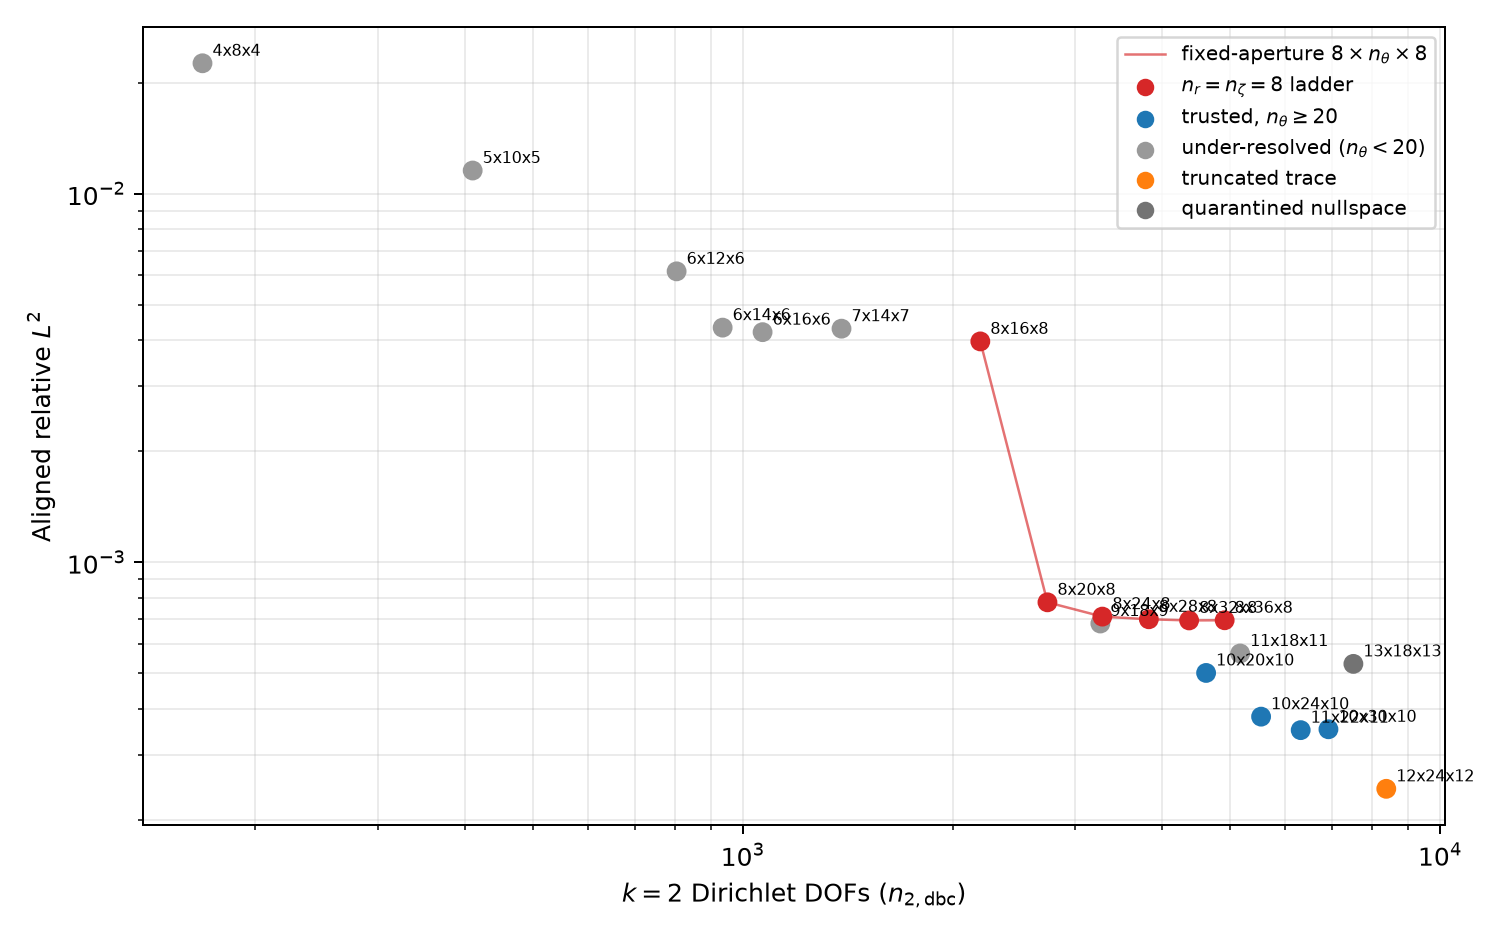
\includegraphics[width=0.88\textwidth]{robust_l2_vs_dofs.png}
  \caption{Aligned relative \(L^2\) versus \(k=2\) Dirichlet DOFs for the
  frozen-tracer evaluation pass shared with Table~\ref{tab:highres}
  (field convergence only).  The red ladder is the fixed-aperture
  \(8\times n_\theta\times8\) series, including \(8\times36\times8\).
  This ranking does \emph{not} predict island fidelity:
  \(8\times32\times8\) has worse \(L^2\) than \(12\times24\times12\) yet
  matches the SIMSOPT island (Section~\ref{sec:width}).}
  \label{fig:l2dofs}
\end{figure}

The isotropic ladder (\(n_r=n_\zeta\), \(n_\theta=2n_r\)) is consistent with
a high-order spatial law \(L^2\sim h^{\,p}\), with fitted \(p\approx4.3\) for
the \(p=3\) spline FEEC spaces.  Island width instead tracks poloidal
elements per lobe (Section~\ref{sec:width}): \(a_{6,3}\) is most efficiently
reduced by increasing \(n_\theta\), not by maximizing total DOFs.

\begin{figure}[htbp]
  \centering
  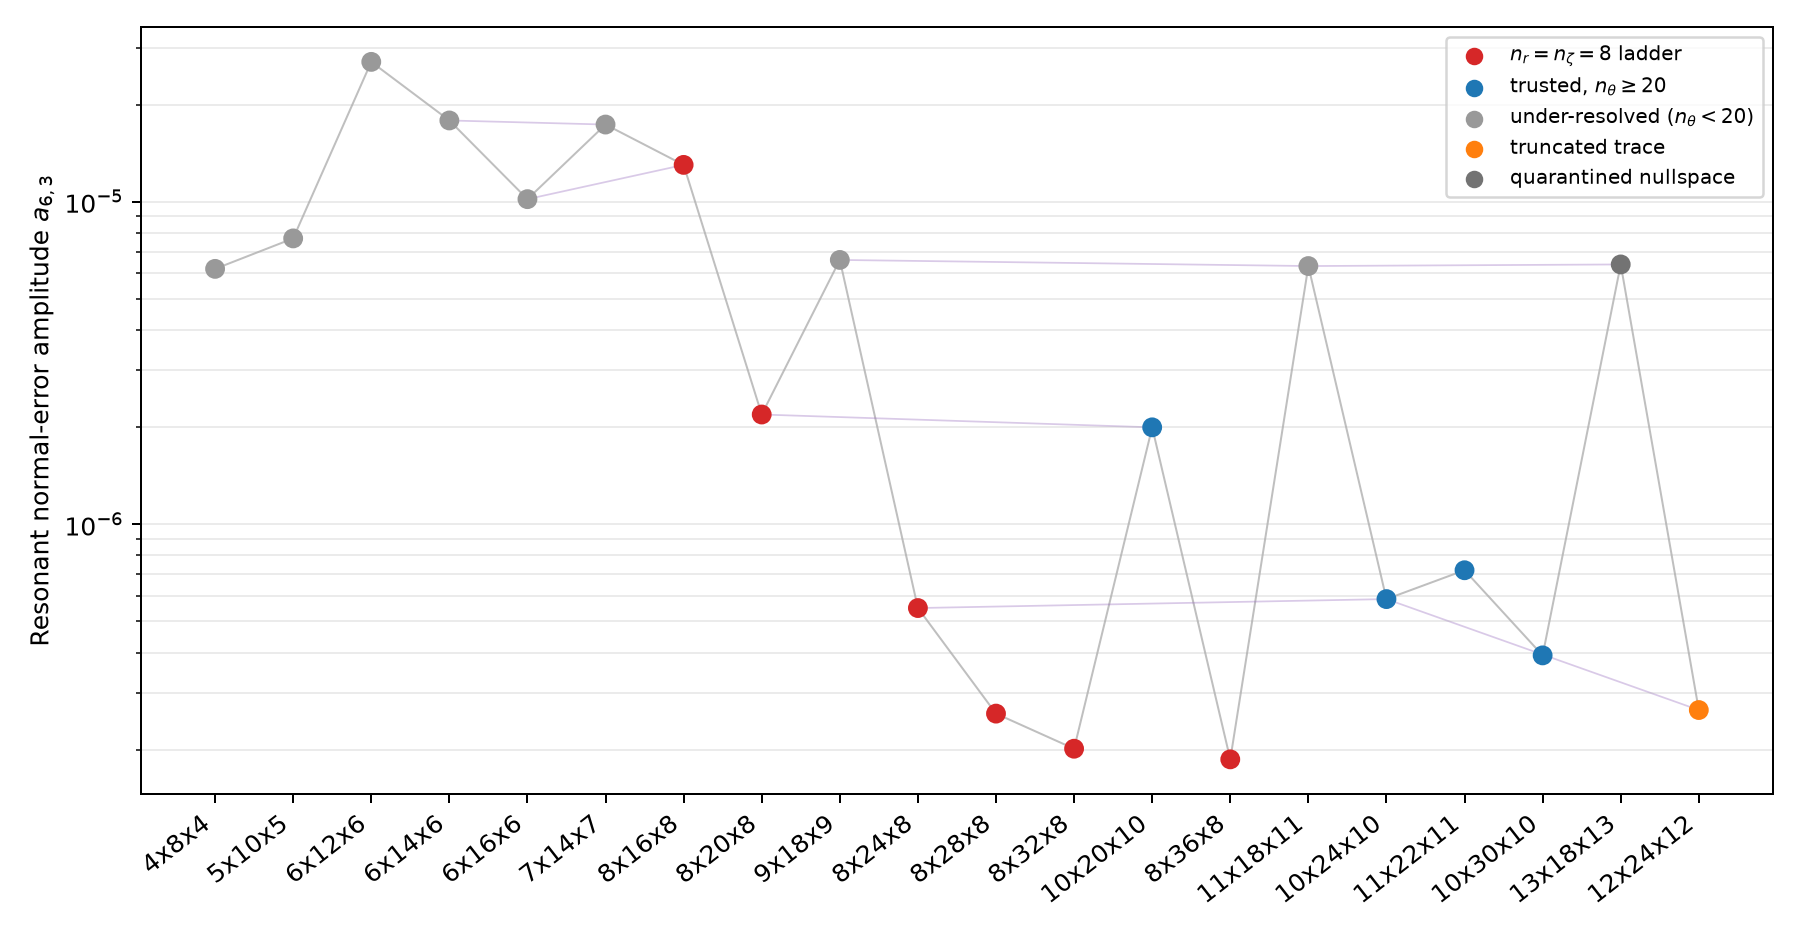
\includegraphics[width=0.88\textwidth]{robust_a63_vs_grid.png}
  \caption{Resonant normal-error amplitude \(a_{6,3}\) on the same
  frozen-tracer records as Figure~\ref{fig:l2dofs}.  Poloidal refinement
  resolves the \(m=6\) error more efficiently than radial/toroidal enrichment
  at fixed \(n_\theta\).}
  \label{fig:a63}
\end{figure}

\section{Island-width convergence}
\label{sec:width}

\subsection{Resonance location}

All resolved grids place \(\iota=1/2\) near \(\rho^\star=0.69\)--\(0.70\) and
converge to a common local \(\iota(\rho)\) profile.  The \(4\times8\times4\)
mesh is the sole location outlier.  Boundary resonant flux
(\(\sim6\times10^{-9}\,B_{\mathrm{rms}}\) on the GVEC \(\rho=1\) surface) and
seed-density bias of the frozen \(16\rho\times6\theta\) protocol
(\(\sim4\%\) on the \(11\times22\times11\) detrended width) are both ruled out
as drivers of residual width gaps on under-resolved grids.

\begin{figure}[htbp]
  \centering
  \begin{subfigure}{0.49\textwidth}
    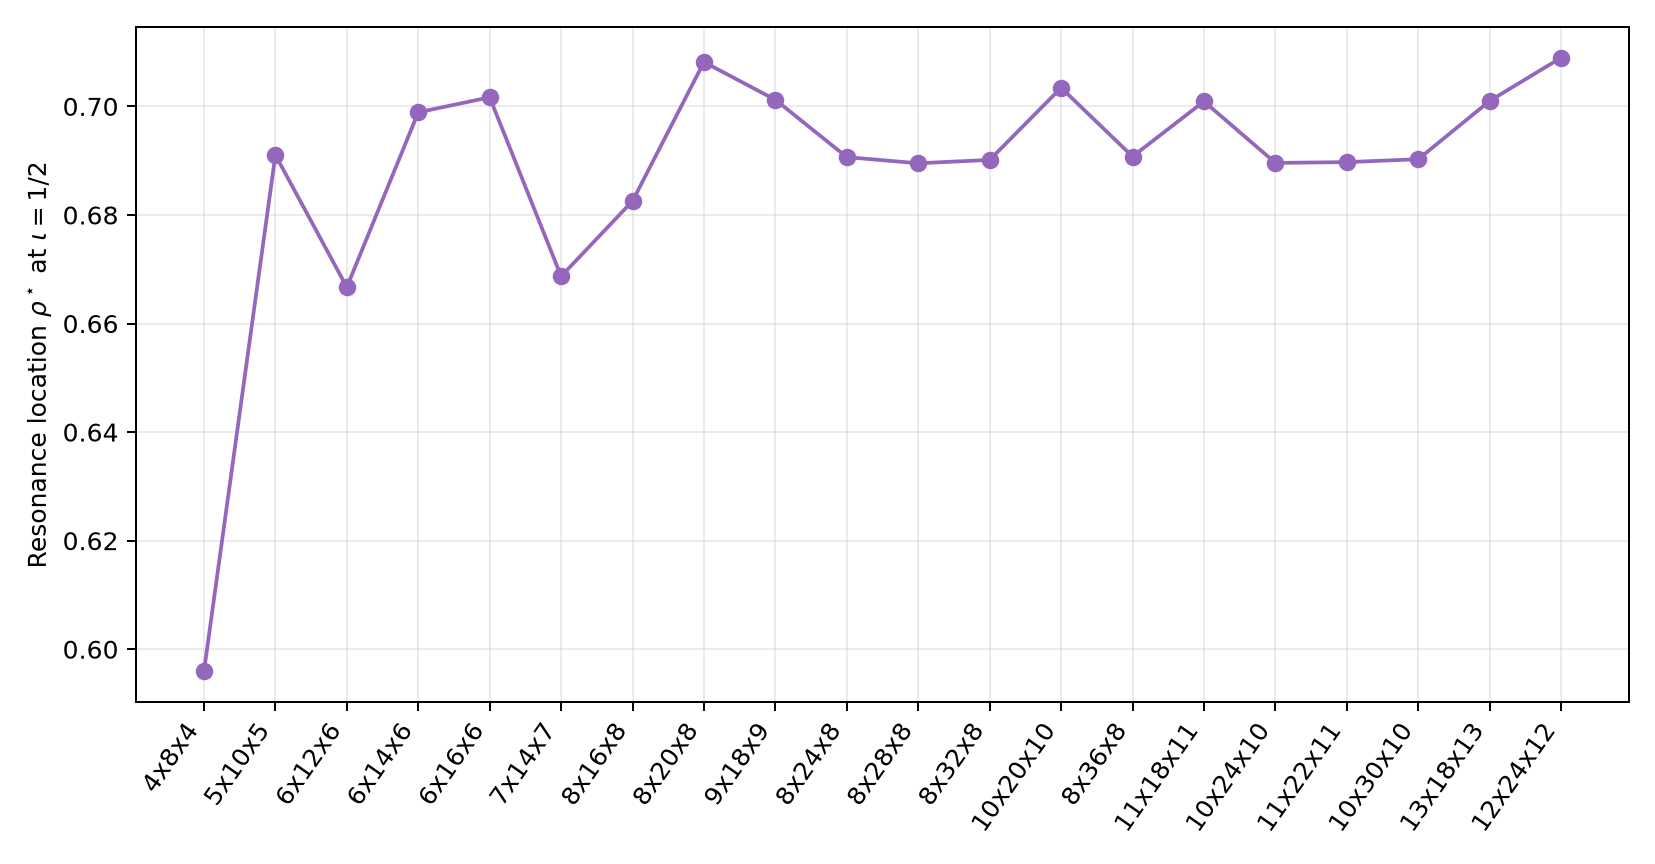
\includegraphics[width=\textwidth]{robust_rho_star_vs_grid.png}
    \caption{Resonance radius.}
  \end{subfigure}
  \hfill
  \begin{subfigure}{0.49\textwidth}
    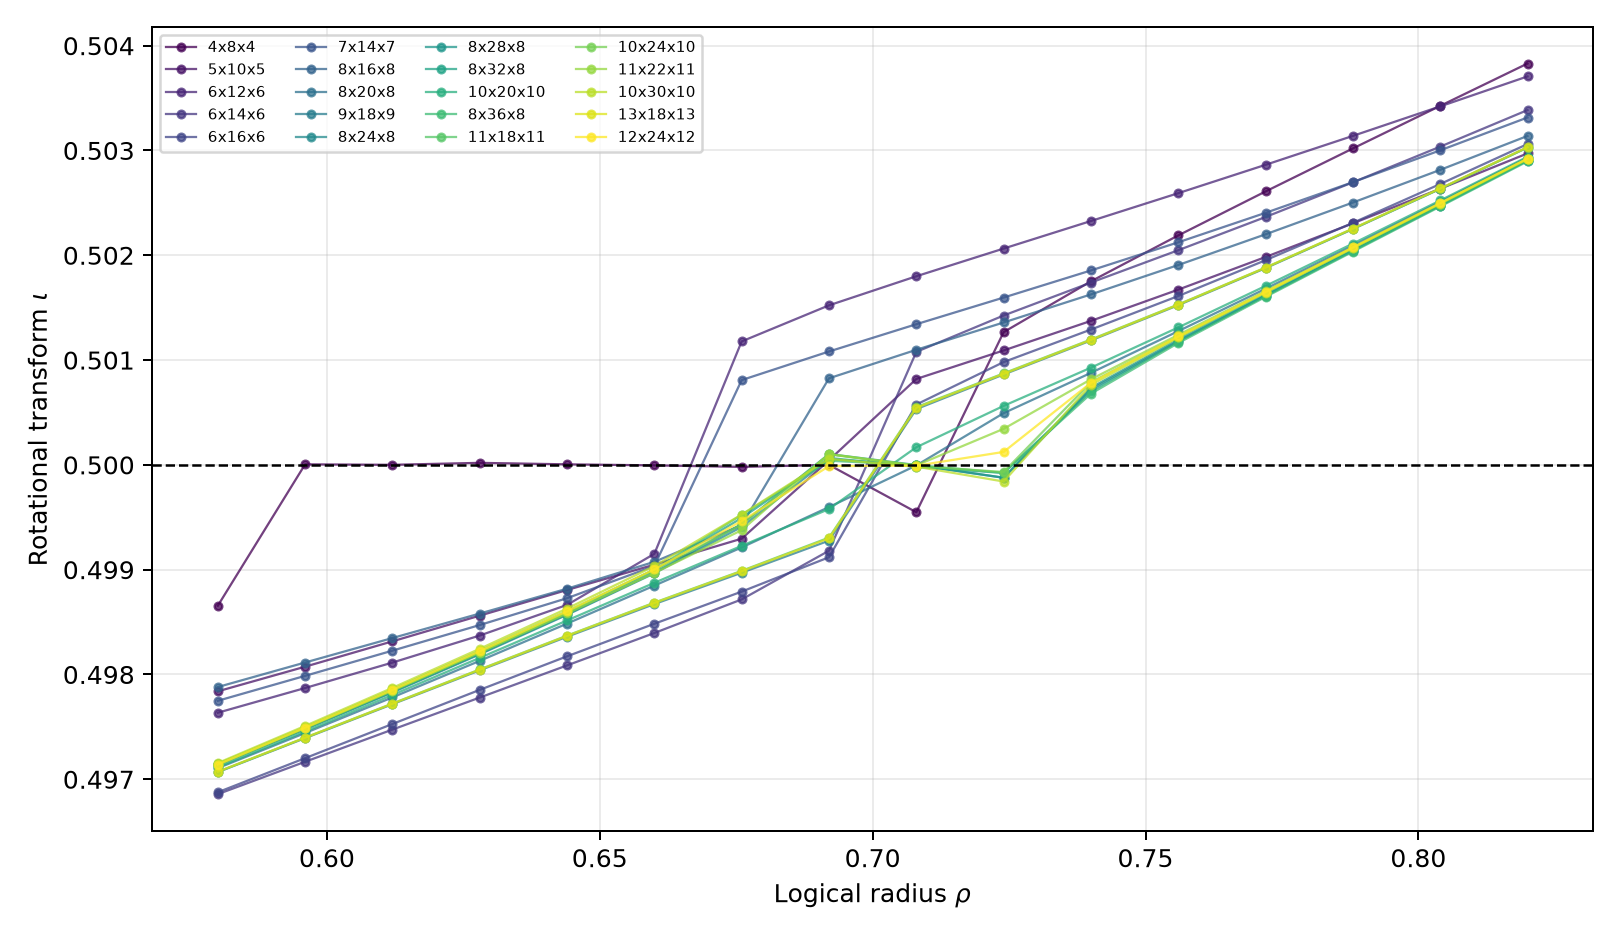
\includegraphics[width=\textwidth]{robust_iota_profiles.png}
    \caption{Transform profiles.}
  \end{subfigure}
  \caption{Fixed-tracer convergence of resonance location and
  \(\iota(\rho)\) through \(\iota=1/2\).}
  \label{fig:robust-location}
\end{figure}

\subsection{Resonant-pitch attribution and the relative width law}
\label{sec:width-bottleneck}

Across the saved fields, the complex resonant radial-pitch harmonic
\(\widehat{B^\rho/B^\zeta}_{6,1}\) at each grid's own \(\iota=1/2\) surface
predicts the traced detrended width through the pendulum law
\[
W = 4\sqrt{\lvert c\rvert\big/\bigl(2\pi\,\lvert\mathrm{d}\iota/\mathrm{d}\rho\rvert\bigr)},
\]
where \(c\) is the complex Fourier coefficient of \(B^\rho/B^\zeta\)
(Figure~\ref{fig:width-attribution}).  With phase
\(\psi=2\pi(6\theta-\zeta)\) on the field-period coordinate and \(\iota\)
reported per full turn, the factor \(2\pi\) is the correct shear
normalization.

The shear cancels in the relative form
\[
\frac{w_{\mathrm{MRX}}}{w_{\mathrm{SIMSOPT}}}
=
\sqrt{\frac{A_{\mathrm{MRX}}}{A_{\mathrm{SIMSOPT}}}},
\]
which is the headline diagnostic (Figure~\ref{fig:elements-per-lobe}).
Trusted grids with at least \(\approx3.3\) poloidal elements per lobe
satisfy this identity to within a few percent; at \(8\times32\times8\)
(\(5.33\) elements/lobe) both the amplitude ratio and the width ratio are
unity against the corrected SIMSOPT reference \(w=0.0501\).

\begin{figure}[htbp]
  \centering
  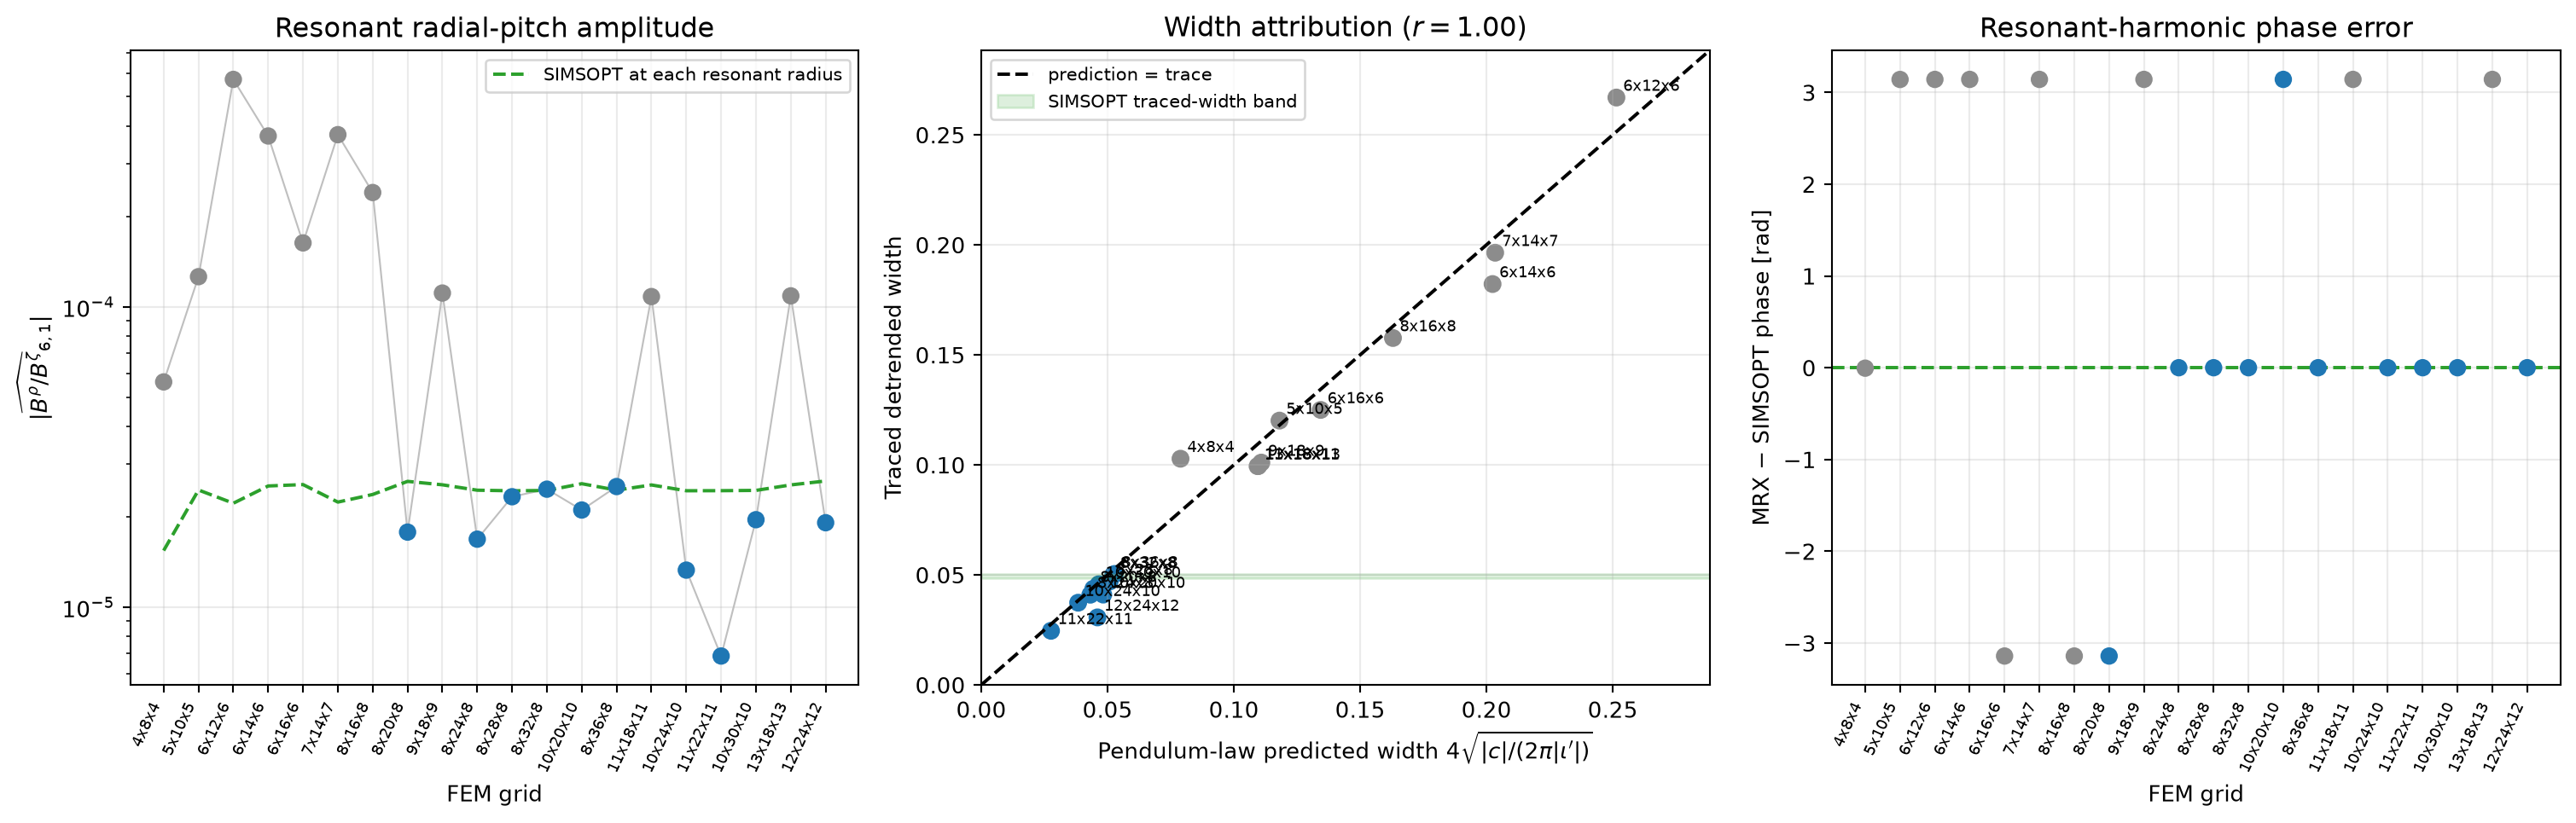
\includegraphics[width=0.96\textwidth]{width_attribution.png}
  \caption{Width attribution.  Resonant pitch amplitudes track poloidal
  resolution; predicted and traced detrended widths agree closely.}
  \label{fig:width-attribution}
\end{figure}

\begin{figure}[htbp]
  \centering
  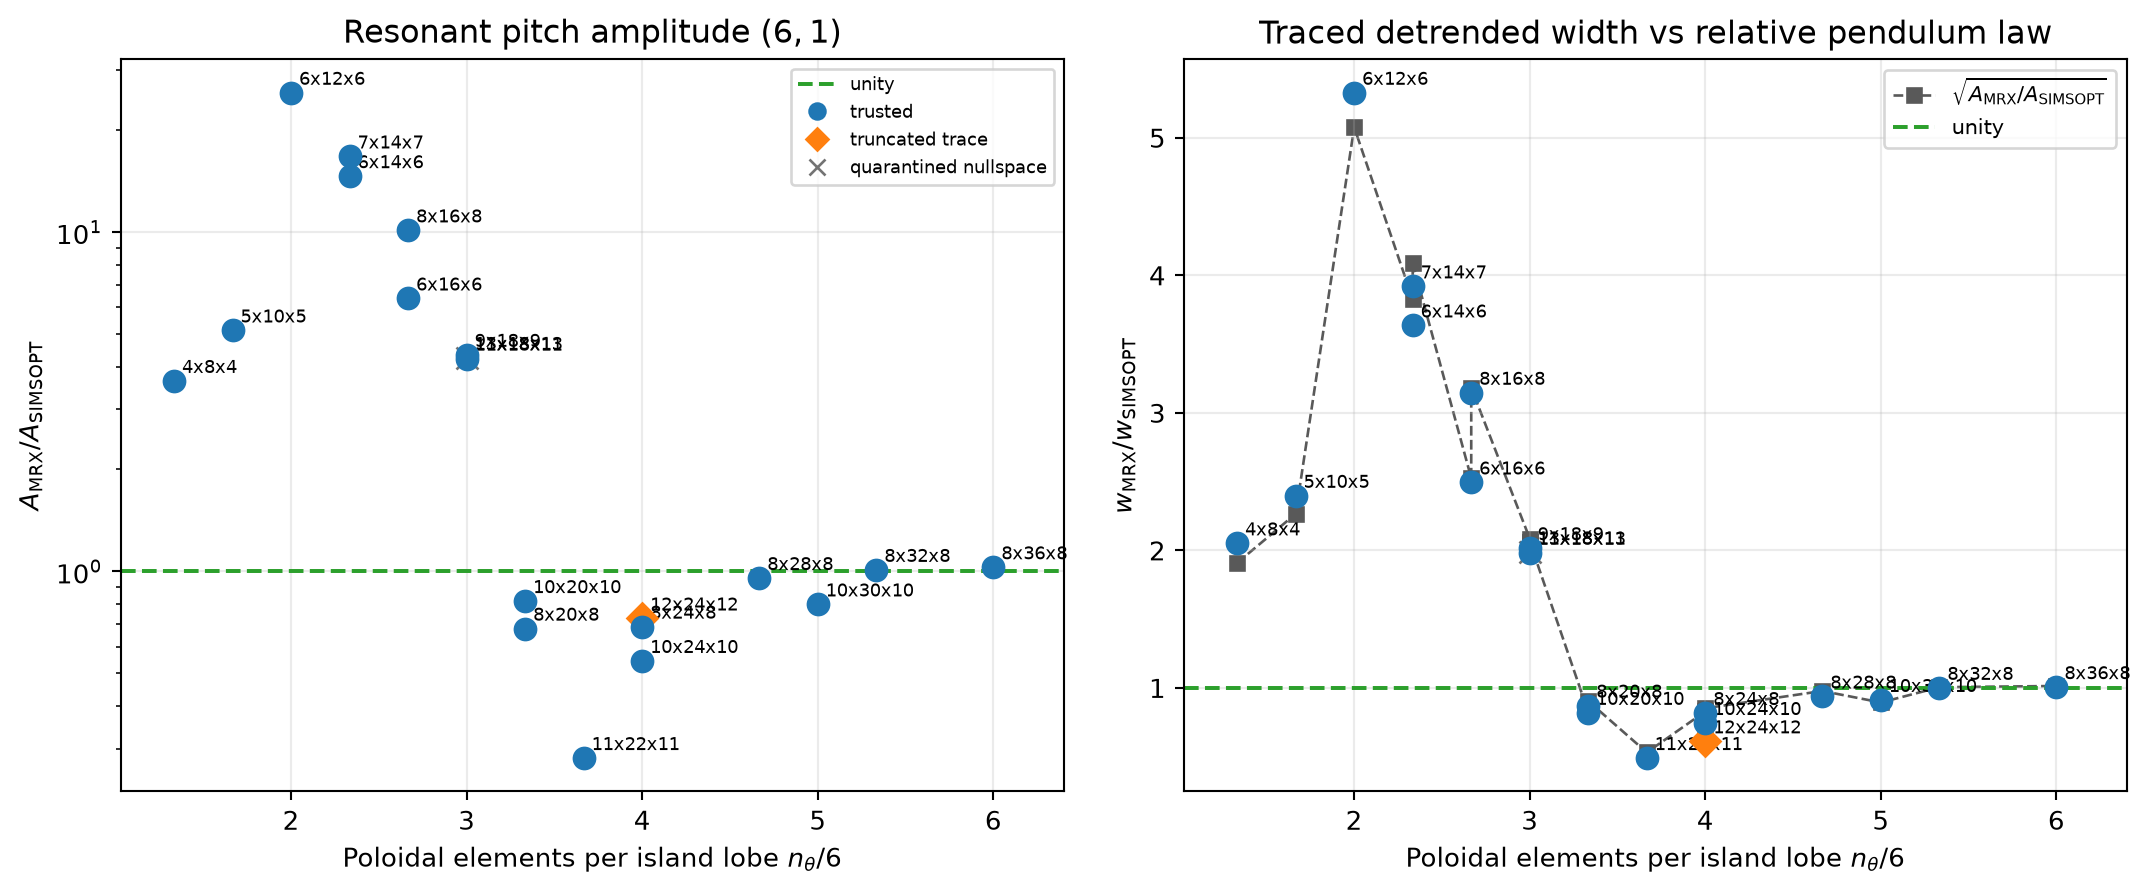
\includegraphics[width=0.96\textwidth]{elements_per_lobe_convergence.png}
  \caption{Island fidelity versus poloidal elements per lobe
  \(n_\theta/6\).  Left: resonant pitch amplitude ratio.  Right: traced
  width ratio overlaid with \(\sqrt{A_{\mathrm{MRX}}/A_{\mathrm{SIMSOPT}}}\).
  Under-resolved grids overshoot; the ratios approach unity near
  \(5.3\) elements/lobe.  Orange markers are truncated traces; grey
  crosses are quarantined nullspaces.}
  \label{fig:elements-per-lobe}
\end{figure}

Aligned \(L^2\) does \emph{not} rank island fidelity.
\(8\times32\times8\) has \(4368\) DOFs and aligned \(L^2=6.95\times10^{-4}\),
worse than \(12\times24\times12\) (\(8376\) DOFs,
\(L^2=2.43\times10^{-4}\)), yet \(8\times32\times8\) matches the SIMSOPT
island while the denser grid's truncated trace does not.  DOF-ordered
plots therefore look non-monotone even when the elements-per-lobe law is
clean.  Two grids are excluded from the headline fit:
\(13\times18\times13\) (dense/iterative M2 overlap \(0.73\), quarantined)
and \(12\times24\times12\) (truncated \(1000\)-turn re-trace).

\subsection{Fixed-aperture poloidal ladder}
\label{sec:8x-ladder}

The decisive test is a six-point ladder at fixed aperture
\(n_\rho=n_\zeta=8\), varying only \(n_\theta\)
(Table~\ref{tab:8x-ladder}, Figure~\ref{fig:elements-per-lobe}).
Under-resolved \(8\times16\times8\) (\(2.67\) elements/lobe) produces a
spurious numerical over-island.  From \(3.33\) elements/lobe upward the
amplitude and width ratios rise toward unity; at \(5.33\) and \(6.00\)
elements/lobe both ratios are \(1.00\)--\(1.03\).  This plateau confirms
convergence rather than a crossing coincidence.

\begin{table}[htbp]
  \centering
  \caption{Fixed-aperture poloidal ladder (\(n_\rho=n_\zeta=8\), frozen
  \(16\rho\times6\theta\times2000\) tracer).  Width ratios use the
  corrected SIMSOPT reference \(w=0.0501\).}
  \label{tab:8x-ladder}
  \begin{tabular}{@{}lrrrrr@{}}
    \toprule
    Grid & el/lobe & DOFs & \(A_{\mathrm{MRX}}/A_{\mathrm{SIMSOPT}}\) &
    \(w_{\mathrm{det}}\) & \(w/w_{\mathrm{SIMSOPT}}\) \\
    \midrule
    \(8\times16\times8\) & 2.67 & 2192 & 10.122 & 0.1576 & 3.146 \\
    \(8\times20\times8\) & 3.33 & 2736 & 0.678 & 0.0437 & 0.872 \\
    \(8\times24\times8\) & 4.00 & 3280 & 0.687 & 0.0410 & 0.818 \\
    \(8\times28\times8\) & 4.67 & 3824 & 0.955 & 0.0470 & 0.938 \\
    \(8\times32\times8\) & 5.33 & 4368 & 1.010 & 0.0501 & 1.001 \\
    \(8\times36\times8\) & 6.00 & 4912 & 1.028 & 0.0504 & 1.006 \\
    \bottomrule
  \end{tabular}
\end{table}

Dense verification is essential on this ladder: at \(8\times36\times8\) the
iterative null vector has M2 overlap only \(0.185\) with the dense
eigenvector, yet the saved dense harmonic still yields the physical island.
The iterative impurity is therefore a solver-health warning, not a
disqualification of the dense-verified field.

\begin{figure}[htbp]
  \centering
  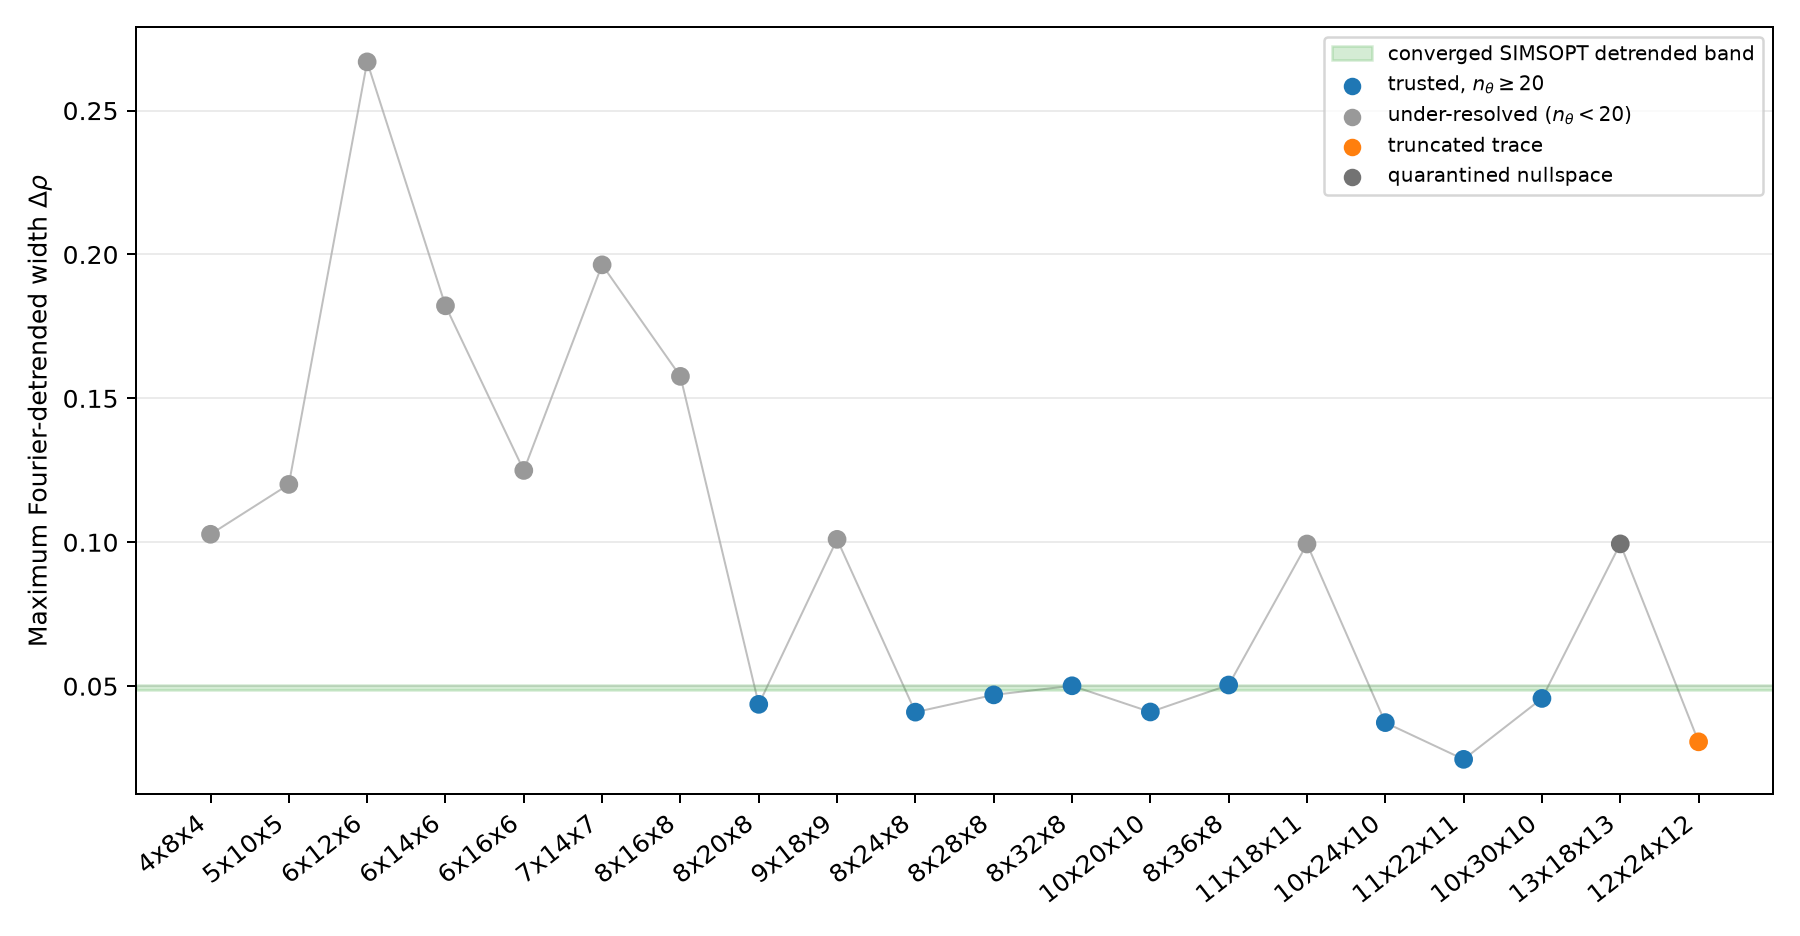
\includegraphics[width=0.88\textwidth]{robust_detrended_width_vs_grid.png}
  \caption{MRX maximum Fourier-detrended width compared with the converged
  SIMSOPT band.  Poloidal resolution removes large numerical over-islands;
  \(8\times32\times8\) and \(8\times36\times8\) sit on the physical reference.}
  \label{fig:robust-detrended}
\end{figure}

\subsection{Manuscript Poincaré comparison}

Figure~\ref{fig:manuscript-poincare} places the converged physical SIMSOPT
chain beside the two highest points of the fixed-aperture ladder.  Logical
\(\zeta=0\) is not the cylindrical plane \(\phi=0\) used by SIMSOPT
(\(|\phi|\) reaches \(3.4\times10^{-2}\,\mathrm{rad}\) on the wavy logical
section); the physical row therefore embeds both fields through the same
Newton-corrected \(\phi=0\) slice.  SIMSOPT used \(32\) radial \(\times\)
\(6\) phase seeds; MRX used the frozen \(16\times6\) protocol.  The physical
panels are a common coordinate embedding, not a claim that the two tracers
recorded identical section events.

\begin{figure}[htbp]
  \centering
  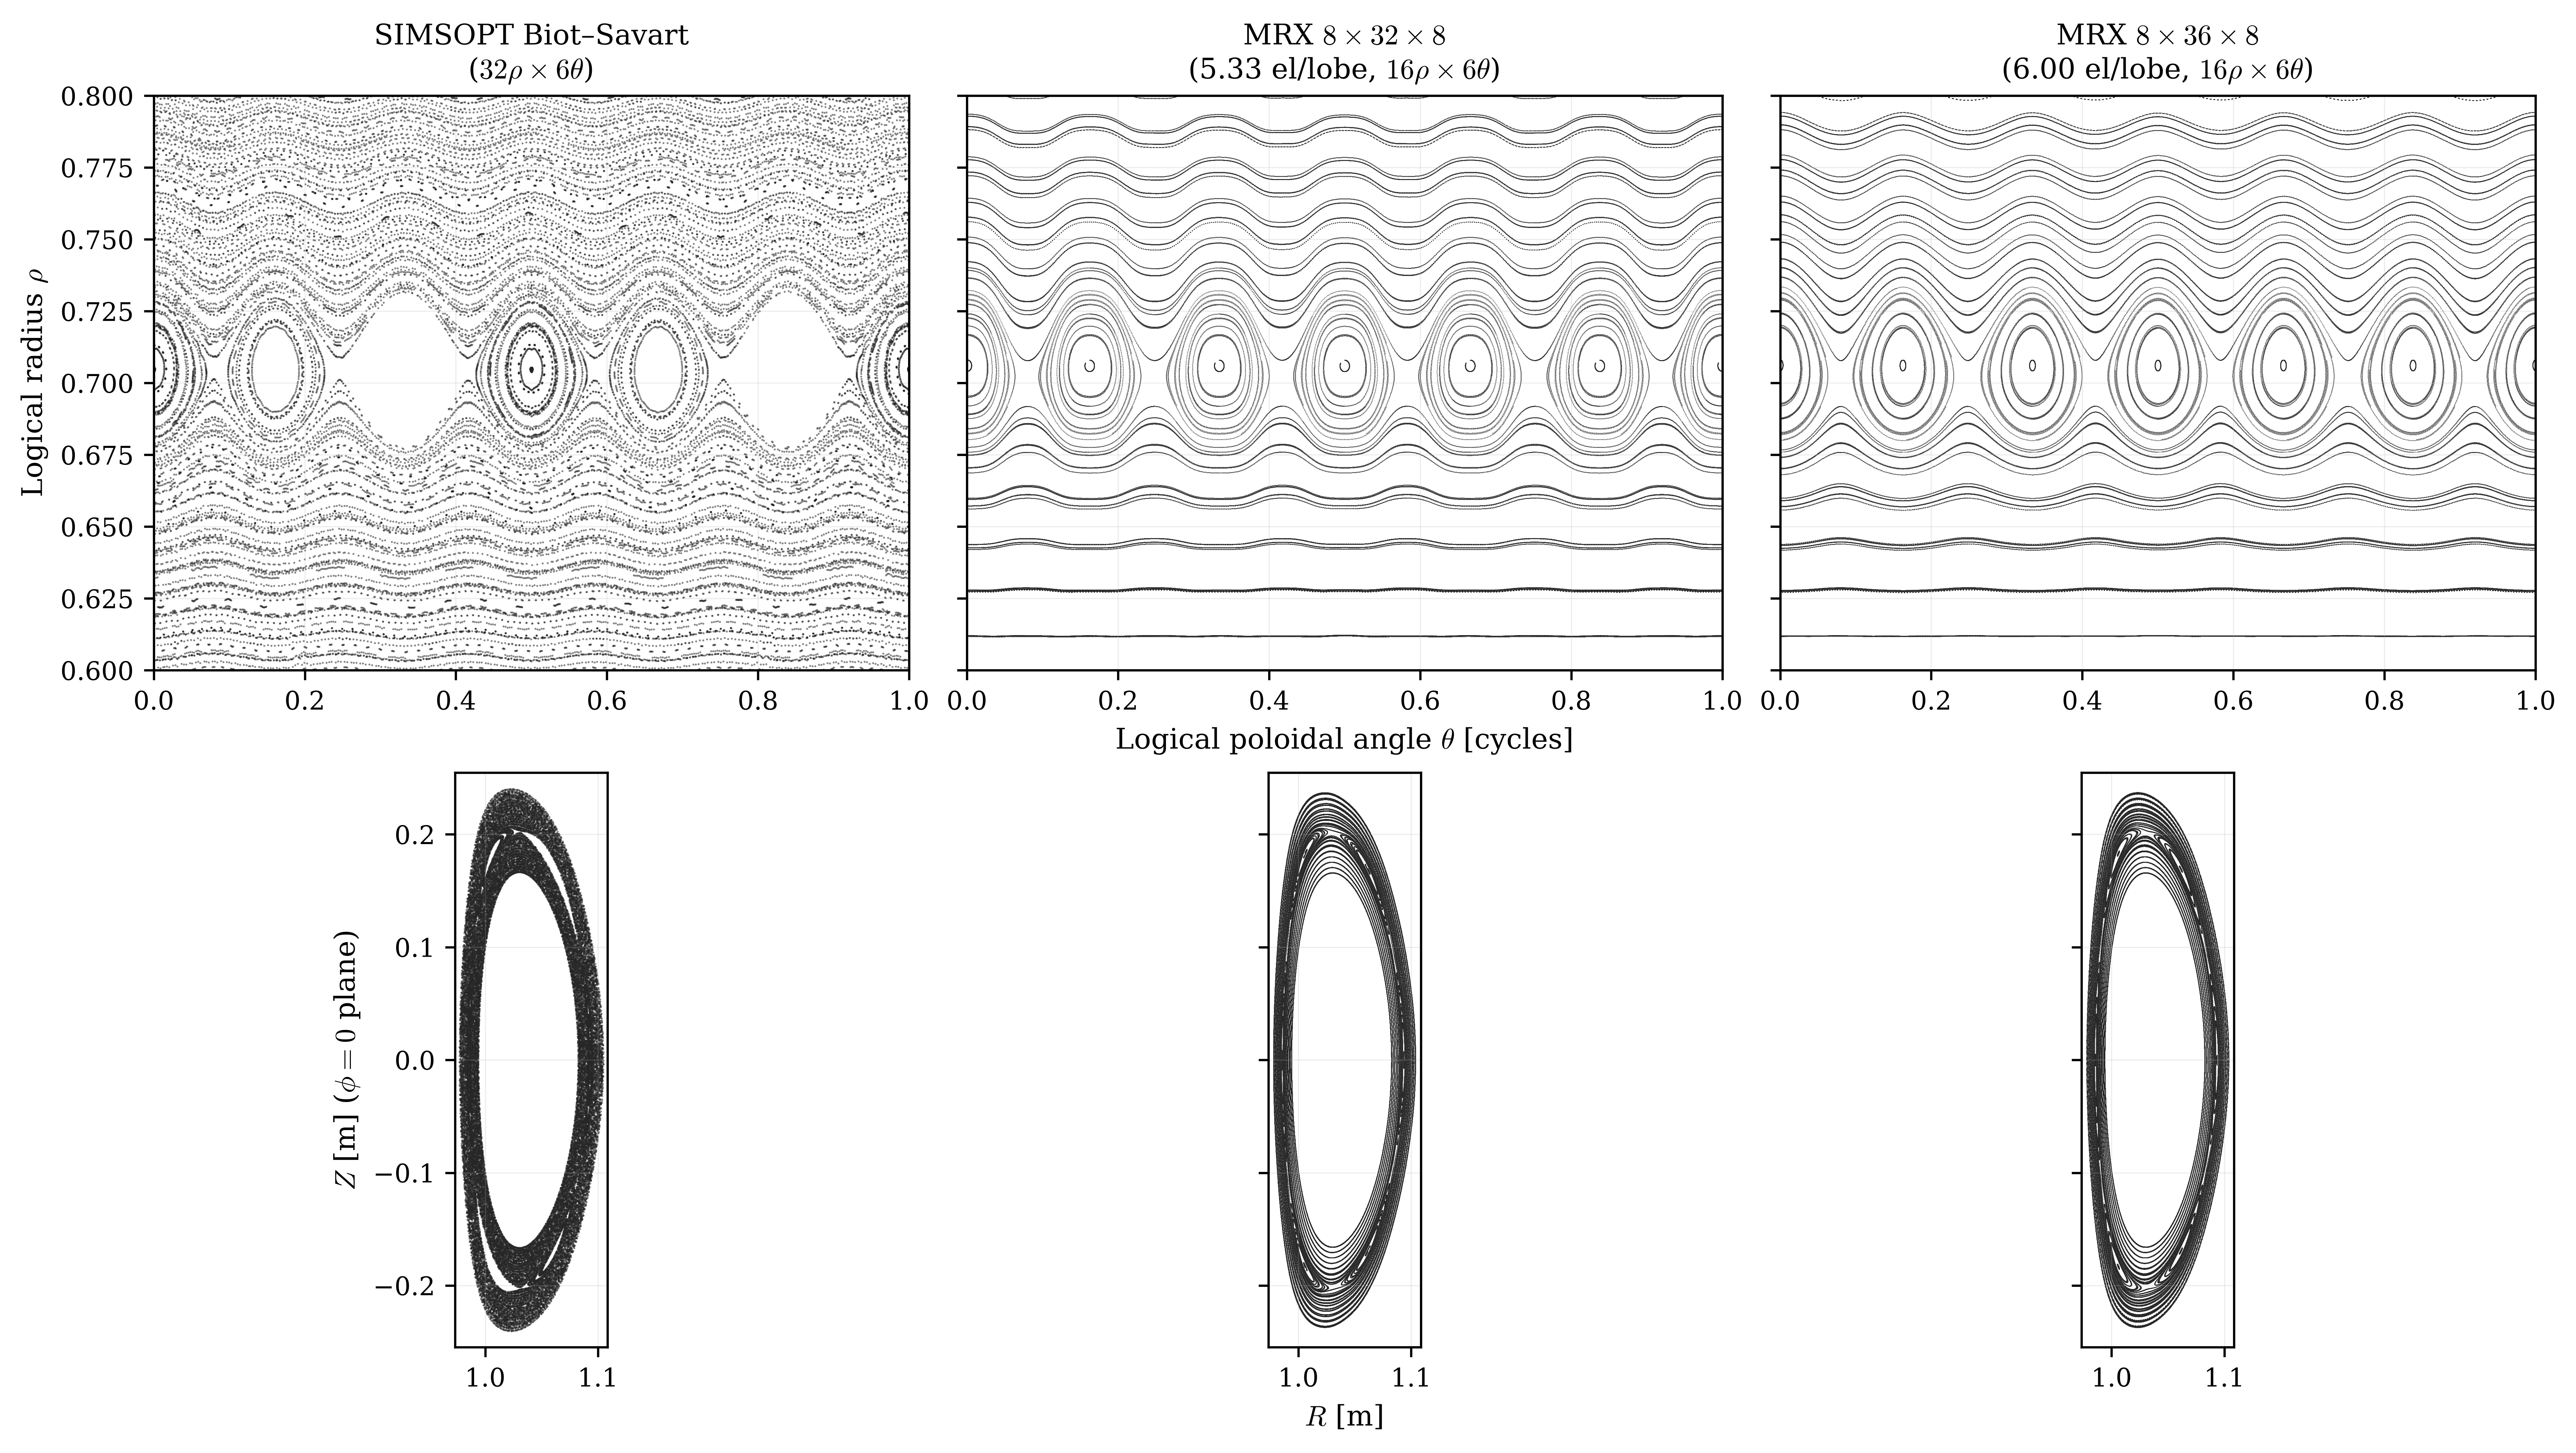
\includegraphics[width=\textwidth]{manuscript_poincare_simsopt_vs_mrx_8x32_8x36.png}
  \caption{High-resolution Poincaré comparison.  Top: logical
  \((\rho,\theta)\) island zoom.  Bottom: trapped and passing orbits in a
  common physical \(\phi=0\) embedding.  Columns are SIMSOPT Biot--Savart
  (\(32\rho\times6\theta\)), MRX \(8\times32\times8\)
  (\(5.33\)~elements/lobe), and MRX \(8\times36\times8\)
  (\(6.00\)~elements/lobe).  At these poloidal resolutions the MRX island
  chain matches the physical SIMSOPT width and location.}
  \label{fig:manuscript-poincare}
\end{figure}

\section{Code changes required}
\label{sec:code}

The following changes were required relative to the original branch to make
the \(L^2\) and island-width demonstrations reliable.  Each item names the
function and the failure mode it fixed.

\paragraph{Dense \texttt{eigh} verification.}
Inexact shift-and-invert inverse iteration can return a vector with high
scalar \(M_2\) overlap but an impure non-harmonic component.  Dense
\texttt{eigh} on the assembled Hodge Laplacian replaces that vector with the
exact discrete harmonic form before any diagnostic is computed.  Without this
step, field \(L^2\) and island width both fail to converge monotonically.
Grids whose iterative warm-start has low dense overlap are quarantined from
headline fits; low overlap of the iterative vector alone remains a
solver-health caveat when the dense-verified field is still usable
(\(8\times36\times8\)).

\paragraph{Exact section crossings
(\texttt{\_exact\_section\_times}).}
Reparameterizing the field-line ODE so that \(\mathrm{d}\zeta/\mathrm{d}t=1\)
makes Poincaré crossings land at known times.  Adaptive-step integrators that
detect zero-crossings of \(\zeta-\zeta_{\mathrm{section}}\) accumulate phase
error over thousands of turns; the exact-time schedule removes that drift.

\paragraph{Bounded-chunk Diffrax batching
(\texttt{\_poincare\_chunk\_size}).}
Batched Diffrax \texttt{Tsit5} is fast when every seed is healthy, but a
single pathological seed forces tiny adaptive steps for the entire batch.
Default chunking uses \(\min(8,n_{\mathrm{seeds}})\); the environment variable
\texttt{MRX\_POINCARE\_CHUNK=1} forces per-seed integration for known bad
grids (the truncated \(12\times24\times12\) re-trace).

\paragraph{\(\phi=0\) slice Newton correction
(\texttt{\_physical\_phi\_zero\_slice},
\texttt{\_logical\_to\_phi\_zero\_rz}).}
SIMSOPT records the cylindrical plane \(\phi=0\); MRX was originally sampled
at logical \(\zeta=0\).  Inverting SIMSOPT hits against the wavy logical
section imposed a spurious radial trend on the SIMSOPT O-points.  Solving for
the logical slice whose mapped points satisfy \(\phi=0\) removes that
artifact and enables a fair physical overlay.

\paragraph{Fourier-detrended width
(\texttt{\_island\_width\_profile}).}
Raw \(\rho_{q95}-\rho_{q05}\) conflates smooth surface-label shape with
island width.  Subtracting poloidal modes 1--4 from \(\rho(\theta)\) before
measuring the spread isolates the resonant deformation and yields the stable
SIMSOPT reference \(w_{\mathrm{phys}}\approx0.050\).

\paragraph{Circulation on the native single-period map.}
\leavevmode\\[-0.35em]
Circulation normalization
\(\alpha=\Gamma_{\mathrm{SIMSOPT}}/\Gamma_{\mathrm{MRX,unit}}\) was first
evaluated after unfolding through the legacy full-torus visualization path
(\path{extend_map_nfp} plus a localized \(k=2\) pushforward).
That toroidal reparameterization does not preserve the \(k=2\) Piola proxy:
\(\Gamma_{\mathrm{MRX}}\) acquired the wrong sign relative to
\(n_{\mathrm{fp}}\) times the single-period value, and \(\alpha/s^\star\)
drifted from \(0.978\) at \(\rho=0.30\) to \(0.939\) at \(\rho=0.95\)
(relative span \(4.0\%\) on grid \(11\times22\times11\)).  The fix integrates
both circulations on the native one-field-period map at the interior loop
\(\rho=0.6\), where the \(n_{\mathrm{fp}}\) factor cancels in the ratio.
After the fix, \(\alpha/s^\star\) is flat to \(5\times10^{-5}\) (finest grid
\(1.000053\)); resolved grids satisfy
\(\lvert\alpha/s^\star-1\rvert\le9.8\times10^{-5}\), and
\(s^\star\)-normalized \(L^2\) shifts by at most \(8.3\times10^{-6}\).

\section{Conclusions}

\begin{enumerate}[leftmargin=1.5em,itemsep=0.25em]
  \item \textbf{Vacuum-field convergence is demonstrated.}  Dense-verified
  aligned \(L^2\) reaches the \(10^{-4}\) range and follows high-order spatial
  convergence.
  \item \textbf{The physical reference is \(w_{\mathrm{phys}}\approx0.050\).}
  It is the seed-robust Fourier-detrended SIMSOPT width
  (\(0.0486\)--\(0.0503\)); no universal trapped-width reference is used.
  \item \textbf{Island convergence is controlled by poloidal elements per
  lobe.}  The relative law
  \(w_{\mathrm{MRX}}/w_{\mathrm{SIMSOPT}}=\sqrt{A_{\mathrm{MRX}}/A_{\mathrm{SIMSOPT}}}\)
  holds for trusted grids.  On the fixed-aperture ladder both ratios reach
  unity at \(8\times32\times8\) and remain there at \(8\times36\times8\)
  (Table~\ref{tab:8x-ladder}).  Aligned \(L^2\) does not rank island
  fidelity.
  \item \textbf{Retain dense verification where topology matters.}  The exact
  discrete harmonic form avoids the iterative impurity described in
  Section~\ref{sec:why}; quarantine grids with M2 overlap
  \(\lesssim0.75\) and caveat truncated traces.
  \item \textbf{Resolve \(m=6\) poloidally before adding other DOFs.}
  Fixed-aperture enrichment in \(n_\theta\) is the appropriate island
  resolution study; increasing radial and toroidal DOFs at fixed poloidal
  resolution does not converge the island.
\end{enumerate}

\end{document}
